%%
%% This is file `sample-sigconf-biblatex.tex',
%% generated with the docstrip utility.
%%
%% The original source files were:
%%
%% samples.dtx  (with options: `sigconf-biblatex')
%% 
%% IMPORTANT NOTICE:
%% 
%% For the copyright see the source file.
%% 
%% Any modified versions of this file must be renamed
%% with new filenames distinct from sample-sigconf-biblatex.tex.
%% 
%% For distribution of the original source see the terms
%% for copying and modification in the file samples.dtx.
%% 
%% This generated file may be distributed as long as the
%% original source files, as listed above, are part of the
%% same distribution. (The sources need not necessarily be
%% in the same archive or directory.)
%%
%%
%% Commands for TeXCount
%TC:macro \cite [option:text,text]
%TC:macro \citep [option:text,text]
%TC:macro \citet [option:text,text]
%TC:envir table 0 1
%TC:envir table* 0 1
%TC:envir tabular [ignore] word
%TC:envir displaymath 0 word
%TC:envir math 0 word
%TC:envir comment 0 0
%%
%%
%% The first command in your LaTeX source must be the \documentclass command.
\documentclass[sigconf,natbib=false]{acmart}

%%
%% \BibTeX command to typeset BibTeX logo in the docs
\AtBeginDocument{%
  \providecommand\BibTeX{{%
    Bib\TeX}}}

%% Rights management information.  This information is sent to you
%% when you complete the rights form.  These commands have SAMPLE
%% values in them; it is your responsibility as an author to replace
%% the commands and values with those provided to you when you
%% complete the rights form.
\setcopyright{none}
\settopmatter{printacmref=false}
% \copyrightyear{2018}
% \acmYear{2018}
% \acmDOI{XXXXXXX.XXXXXXX}



%%
%% Submission ID.
%% Use this when submitting an article to a sponsored event. You'll
%% receive a unique submission ID from the organizers
%% of the event, and this ID should be used as the parameter to this command.
%%\acmSubmissionID{123-A56-BU3}

%%
%% For managing citations, it is recommended to use bibliography
%% files in BibTeX format.
%%
%% You can then either use BibTeX with the ACM-Reference-Format style,
%% or BibLaTeX with the acmnumeric or acmauthoryear sytles, that include
%% support for advanced citation of software artefact from the
%% biblatex-software package, also separately available on CTAN.
%%
%% Look at the sample-*-biblatex.tex files for templates showcasing
%% the biblatex styles.
%%


%%
%% The majority of ACM publications use numbered citations and
%% references, obtained by selecting the acmnumeric BibLaTeX style.
%% The acmauthoryear BibLaTeX style switches to the "author year" style.
%%
%% If you are preparing content for an event
%% sponsored by ACM SIGGRAPH, you must use the acmauthoryear style of
%% citations and references.
%%
%% Bibliography style
\RequirePackage[
  datamodel=acmdatamodel,
  style=acmnumeric,
  ]{biblatex}

%% Declare bibliography sources (one \addbibresource command per source)
\addbibresource{software.bib}
\addbibresource{sample-base.bib}

\newcommand{\todo}[1]{\textcolor{red}{#1}}

%%
%% end of the preamble, start of the body of the document source.
\begin{document}

%%
%% The "title" command has an optional parameter,
%% allowing the author to define a "short title" to be used in page headers.
\title{FPGA-Accelerated NAT Project Report}

%%
%% The "author" command and its associated commands are used to define
%% the authors and their affiliations.
%% Of note is the shared affiliation of the first two authors, and the
%% "authornote" and "authornotemark" commands
%% used to denote shared contribution to the research.
\author{Yongtong Wu}
% \authornote{Both authors contributed equally to this research.}
% \email{trovato@corporation.com}
% \orcid{1234-5678-9012}
% \author{G.K.M. Tobin}
% \authornotemark[1]
\email{wuyongtong@stu.pku.edu.cn}
\affiliation{%
  \institution{Peking University}
  % \streetaddress{P.O. Box 1212}
  % \city{Beijing}
  % \state{Beijing}
  \country{China}
  % \postcode{43017-6221}
}

\author{Rilin Huang}
\email{2100013095@stu.pku.edu.cn}
\affiliation{%
  \institution{Peking University}
  \country{China}
}

\author{Jialiang Zhang}
\email{2100012902@stu.pku.edu.cn}
\affiliation{%
  \institution{Peking University}
  \country{China}
}

% \author{Aparna Patel}
% \affiliation{%
%  \institution{Rajiv Gandhi University}
%  \streetaddress{Rono-Hills}
%  \city{Doimukh}
%  \state{Arunachal Pradesh}
%  \country{India}}

% \author{Huifen Chan}
% \affiliation{%
%   \institution{Tsinghua University}
%   \streetaddress{30 Shuangqing Rd}
%   \city{Haidian Qu}
%   \state{Beijing Shi}
%   \country{China}}

% \author{Charles Palmer}
% \affiliation{%
%   \institution{Palmer Research Laboratories}
%   \streetaddress{8600 Datapoint Drive}
%   \city{San Antonio}
%   \state{Texas}
%   \country{USA}
%   \postcode{78229}}
% \email{cpalmer@prl.com}

% \author{John Smith}
% \affiliation{%
%   \institution{The Th{\o}rv{\"a}ld Group}
%   \streetaddress{1 Th{\o}rv{\"a}ld Circle}
%   \city{Hekla}
%   \country{Iceland}}
% \email{jsmith@affiliation.org}

% \author{Julius P. Kumquat}
% \affiliation{%
%   \institution{The Kumquat Consortium}
%   \city{New York}
%   \country{USA}}
% \email{jpkumquat@consortium.net}

%%
%% By default, the full list of authors will be used in the page
%% headers. Often, this list is too long, and will overlap
%% other information printed in the page headers. This command allows
%% the author to define a more concise list
%% of authors' names for this purpose.
\renewcommand{\shortauthors}{Wu et al.}

% \begin{abstract}
%   Our abstract here.
% \end{abstract}

\maketitle

\section{Introduction}

% Motivation+problem statement

% Prior work

% Key ideas

% Evaluation results

% Contribution summary

% \textbf{Background.}
NAT is a common network function between local-area network (LAN) and wide-area
network (WAN). 
It tracks L4 connections (i.e. TCP and UDP), translates IP addresses and ports to 
provide transparent address reuse for different clients in LAN.
Implementing NAT in software is convenient, but the massive data traffic (10Gbps or higher) will incur luxurious CPU waste and high packet latency. Therefore, it's common to offload NAT down into hardware such as switches and network interface cards (NIC). 
However, switches and NICs are usually implemented via application-specific integrated circuit (ASIC) which requires a long and expensive cycle from design to production. That makes vendors refuse to put such function into some products with a small audience, such as performant wireless NIC. 



\textbf{Motivation \& key ideas.} 
Under the circumstances above, the Field Programmable Gate Array (FPGA) comes into consideration naturally. 
It allows users to implement custom hardware logic including NAT. Therefore, in this project, we explore the possibility of implementing NAT in FPGA and show the performance gain from hardware-oriented design. 

\textbf{Prior works.} We survey prior works including other hardware offloading approaches and advanced NAT designs. Programmable switches with P4 language support line-rate match-action processing by which NAT can be implemented naturally. 
\footnote{https://github.com/p4lang/switch/blob/master/p4src/nat.p4}
Some high-performance NICs such as Nvidia (Mellanox) ConnectX-4/5/6 can support NAT offloading itself with proper configuration. However, they are all wired NICs for the data center network.
There are also already some trials to implement NAT on FPGA such as the NetFPGA platform. More details can be found at the footnote link.
\footnote{https://www.cl.cam.ac.uk/~osc22/docs/edv10\_nat\_fpga.pdf}

\textbf{Evaluation Results.} In our evaluation, FPGA-based NAT shows up to 7.7\% performance gain in throughput than software-based NAT and better scalability over connection numbers (i.e. the load factor).

\subsection{Contribution Summary}
\begin{itemize}
    \item Exploration and System Design: Yongtong Wu
    \item Hardware Impl. and Testing: Rilin Huang, Yongtong Wu
    \item Software and Testbed Configuration: Jialiang Zhang
    \item Evaluation \& Live Demo Video: Yongtong Wu
    \item Poster: Jialiang Zhang
    \item Report Writing: Rilin Huang, Yongtong Wu
\end{itemize}


\section{System Design}
\begin{figure*}[ht]
    \centering
    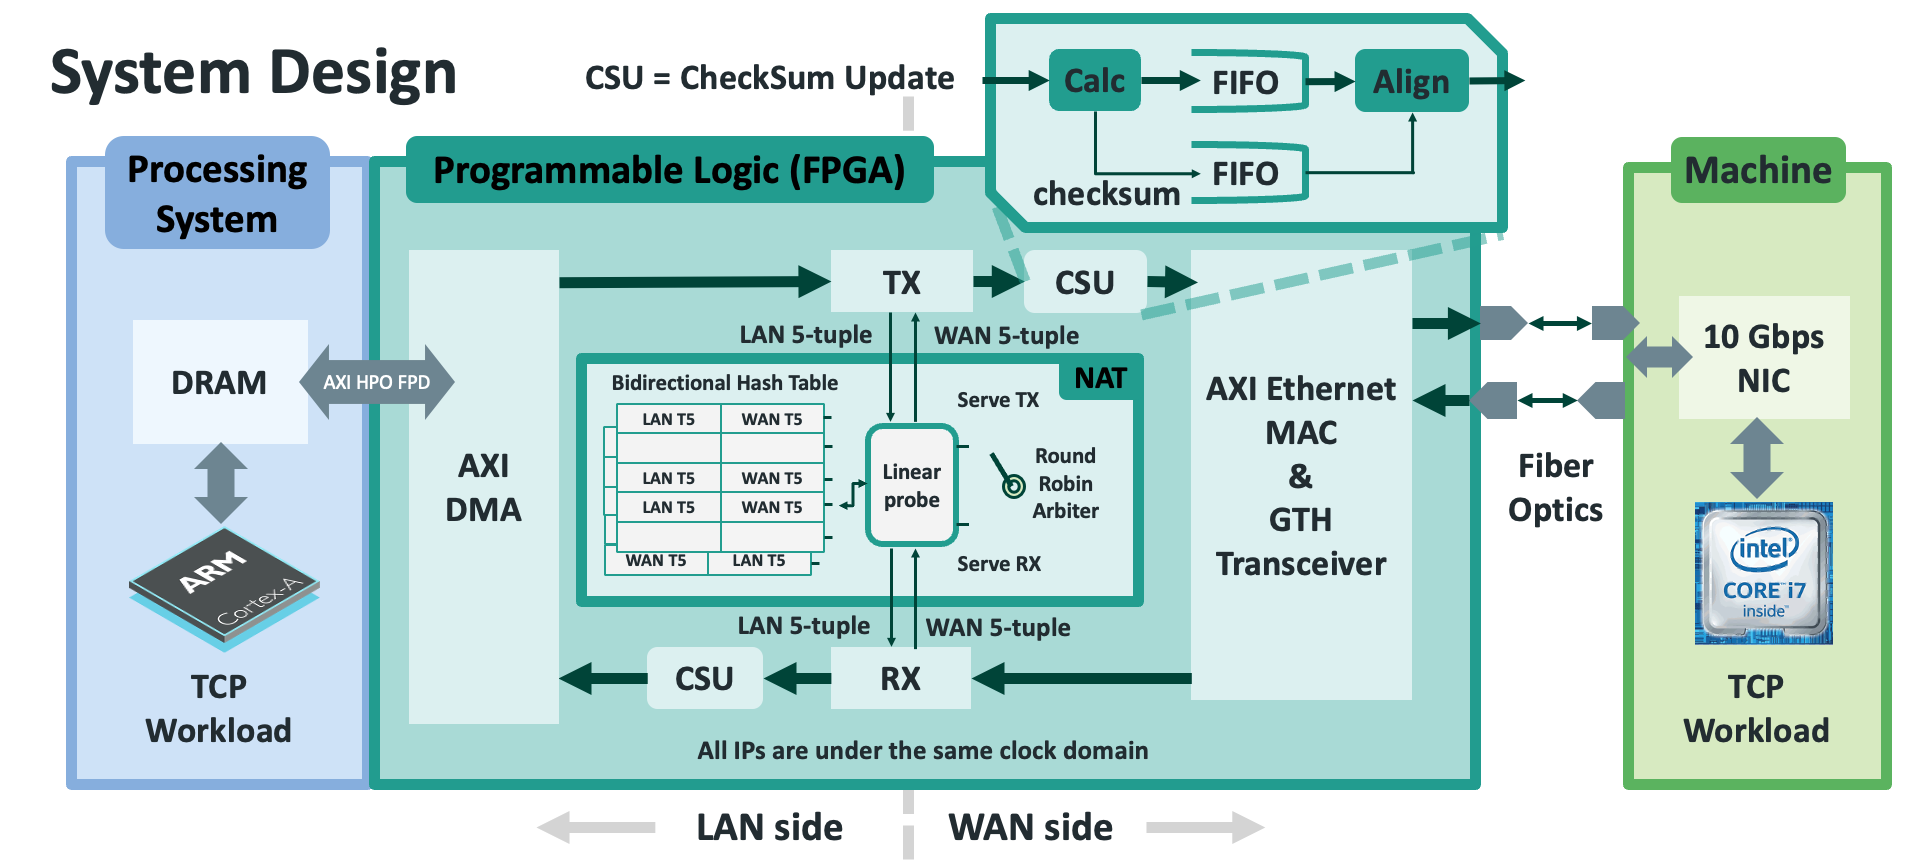
\includegraphics[width=\linewidth]{images/design.png}
    \caption{System Design}
    \label{fig:design}
    \Description{}
\end{figure*}

In this section, we present our system design, which is based on the official example of the Ethernet 10/25G system of Xilinx (referred to as the original design hereafter) \footnote{https://github.com/Xilinx-Wiki-Projects/ZCU102-Ethernet/tree/main/2019.2/pl\_eth\_10g}.

\subsection{Original Block Design}
Before delving into our design, it is essential to provide an overview of the organization of the original design for contextual understanding.

\textbf{Components.} The design integrates the Processing System (PS) and Programmable Logic (PL). The PS in ZCU102 includes four ARM Cortex-A53 processors, capable of handling general-purpose computing tasks and providing control for the entire system. The PL is responsible for implementing custom hardware logic, including components such as DMA, MAC, and GTH, which collectively form a 10GbE network interface on the ZCU102 evaluation board. A Xilinx handmade Linux driver is employed to drive this interface on the PS.

We detail the functions of the components implemented in PL as follows:

\begin{itemize}
    \item \textbf{DMA (Direct Memory Access):} Efficiently transfers data between memory and peripherals without involving the processor, enhancing data throughput and offloading data transfer tasks from the processor.
    \item \textbf{MAC (Media Access Control):} Manages the communication protocol for the Ethernet interface, handling frame formatting, addressing, error detection, and other protocol-related tasks.
    \item \textbf{GTH (Gigabit Transceivers):} Facilitates high-speed serial data communication, enabling the transmission and reception of data at gigabit rates.
\end{itemize}

\textbf{Data Flow.} MAC and GTH handle the transmission of data between the FPGA and the external network. Upon receiving incoming data from MAC and GTH, DMA takes control of the data transfer process and moves it into the designated memory location, allowing further processing by the processor or other system components.

\textbf{AXI4-Stream Signals.} Most signals between the modules adopt the AXI4-Stream protocol, with interfaces appearing in pairs - the slave port (starting with \verb|s_|) and the master port (starting with \verb|m_|). The \verb|ready| signal of the slave and the \verb|valid| signal of the master constitute the primary handshake mechanism, indicating a data transfer when both signals are active.

The exact definitions of these AXI4-Stream signals are as follows:

\begin{itemize}
    \item \verb|s_axis_tdata[63:0]|: Data bus received from the master device, conveying data across the interface.
    \item \verb|s_axis_tkeep[7:0]|: Byte qualifier received from the master device, indicating whether corresponding bytes of the data bus are part of the data stream. A low level indicates an invalid byte.
    \item \verb|s_axis_tvalid|: Signal received from the master device, indicating a valid data transfer.
    \item \verb|s_axis_tlast|: Signal received from the master device, marking the last data transfer and indicating the boundary of the data stream.
    \item \verb|s_axis_tready|: Signal sent to the master device, indicating its readiness to accept a data transfer in the current clock cycle.
    \item \verb|m_axis_tdata[63:0]|: Data bus sent to the slave device, providing data across the interface.
    \item \verb|m_axis_tkeep[7:0]|: Byte qualifier sent to the slave device, indicating whether corresponding bytes of \verb|m_axis_tdata| are part of the data stream. A low level indicates an invalid byte.
    \item \verb|m_axis_tvalid|: Signal sent to the slave device, indicating the reception of a valid data transfer.
    \item \verb|m_axis_tlast|: Signal sent to the slave device, marking the last data transfer and indicating the boundary of the data stream.
    \item \verb|m_axis_tready|: Signal received from the slave device, indicating its readiness to send a data transfer in the current clock cycle.
\end{itemize}

\subsection{TX and RX}
Building upon the original block design, we introduce TX and RX to intercept communication between the MAC/GTH and DMA. TX intercepts communication from DMA to MAC/GTH, while RX intercepts communication from MAC/GTH to DMA. Both TX and RX assess whether an incoming packet is a TCP packet.

If the packet is not a TCP packet, TX and RX simply forward the packet. However, if the packet is a TCP packet, TX and RX extract the 5-tuple information, send it to the NAT IP, wait for a 5-tuple response from NAT IP, and upon receiving the response, modify the packet header according to the received 5-tuple before forwarding the packet.

\subsection{NAT IP}
We introduce a Network Address Translation (NAT) IP to assist TX and RX in modifying the IP and TCP headers of packets based on NAT rules. The NAT IP maintains a bidirectional hash table to store mappings between LAN 5-tuple and WAN 5-tuple. Communication with TX and RX occurs through a simple interface.

\textbf{Hash Function:} The NAT IP employs XOR operation on the 5-tuple \emph{(source IP, source port, destination IP, destination port, protocol)} as its hash function, providing a quick and effective method for generating hash values.

\textbf{Linear Probing:} To handle conflicts within the hash table, the NAT IP utilizes linear probing as a collision resolution strategy. In case of a hash collision, the algorithm linearly searches for the next available slot in the hash table until an empty slot is found.

\textbf{Bidirectional Hash Table:} Our NAT IP incorporates two hash tables - one for the mapping from LAN 5-tuple to WAN 5-tuple and the other for the reverse mapping.

For packets from LAN to WAN, the NAT IP computes the hash value of the LAN 5-tuple, searches for a matching entry in the hash table, allocates a new public port if no entry is found, and modifies the packet header accordingly. If a matching entry is found, the NAT IP replaces \emph{(source IP, source port)} of the packet with \emph{(public IP, public port)} in the corresponding WAN 5-tuple.

For packets from WAN to LAN, the NAT IP can modify the packet header based on the mapping from WAN 5-tuple to LAN 5-tuple.

\textbf{Round Robin Arbiter:} To avoid conflicts arising from concurrent access to the bidirectional hash table by TX and RX, a Round Robin Arbiter is employed in the NAT IP to control access to the hash table. Two signals, $ready\_tx$ and $ready\_rx$, determine which requester should be served. Each ready signal is unset only in the next cycle after the end of service for the corresponding requester, ensuring fair access control to the bidirectional hash table and mitigating synchronization issues between TX and RX.

\subsection{CSU IP}
The CSU (Checksum Update) IP is a custom core that recalculates the IP and TCP checksums of packets after the NAT IP modifies the 5-tuples. This recalibration is essential as sanity checks in hardware and software validate these checksums. Mismatched checksums result in the silent dropping of the packet.

The CSU IP comprises four sub-IPs: Calc, FIFO1, FIFO2, and Align. The Calc module computes the new checksum value based on the modified packet and outputs the new checksum value and the original packet to FIFO1 and FIFO2, respectively. FIFO1 and FIFO2 serve as two FIFO buffers that store the new checksum value and the original packet, awaiting processing by the Align module. The Align module writes the new checksum value into the TCP header of the packet, extracting data from FIFO1 and FIFO2 to locate the TCP checksum field.

\subsection{Put It All Together}
All components of our system design collaborate to achieve the functionality of a hardware-based NAT system, as depicted in Figure \ref{fig:design}. Their clocks are synchronized with \emph{tx\_clk\_out} of MAC/GTH (156 MHz, achieving 10 Gbps with a 64-bit data bus).

Incoming TCP packets undergo the following workflow:
(1) RX extracts the IP and TCP headers from the \emph{s\_axis\_tdata} signal, forming a 5-tuple.
(2) RX sends this 5-tuple to the NAT IP core via a simplified interface with a 5-tuple and a valid signal.
(3) After sending the 5-tuple, RX blocks its input by setting the \emph{s\_axis\_tdata} signal to 0, indicating its inability to accept new data. Simultaneously, RX awaits a response from the NAT IP core.
(4) Upon receiving a new 5-tuple from the NAT IP core, RX modifies the packet header accordingly and resumes normal data reception.
(5) All packets from RX are then forwarded to CSU for TCP checksum updating before being processed by DMA.

\section{Implementation}

We show our implementation in this section, including the testbed setting, the whole workflow, and implementation results such as code lines and FPGA resource consumption. We implement our design based on Xilinx's official example of the Ethernet 10/25G system.
\subsection{Testbed Configuration}
We implemented our NAT with AMD (Xilinx) Zynq UltraScale+ MPSoC ZCU102 (called the board later). The evaluation setup includes the board, a router, and a desktop machine.
The board runs Linux 4.19.0 on its four PS ARM cores. 
The desktop runs Ubuntu 18.04 equipped with Intel i7-9700K and an NVIDIA (Mellanox) ConnectX-3, 
whose line rate reaches 10Gbps, with \verb|mlx4| driver version 4.14.142-ubwins+. The MTU is configured as 9000B to get full performance.
The performance of the router is not critical since we only use it to ssh connect to the board.





\textbf{Network Topology.} 
The board's 1Gbps interface and the on-board NIC of the desktop are both connected to the router and are configured under the same subnet. 
For the data plane, we connect the 10Gbps interface of the board and an interface of ConnectX-3 back-to-back to fully investigate the potential of our FPGA NAT.

\subsection{Implementation Workflow}


\begin{figure*}[h]
    \centering
    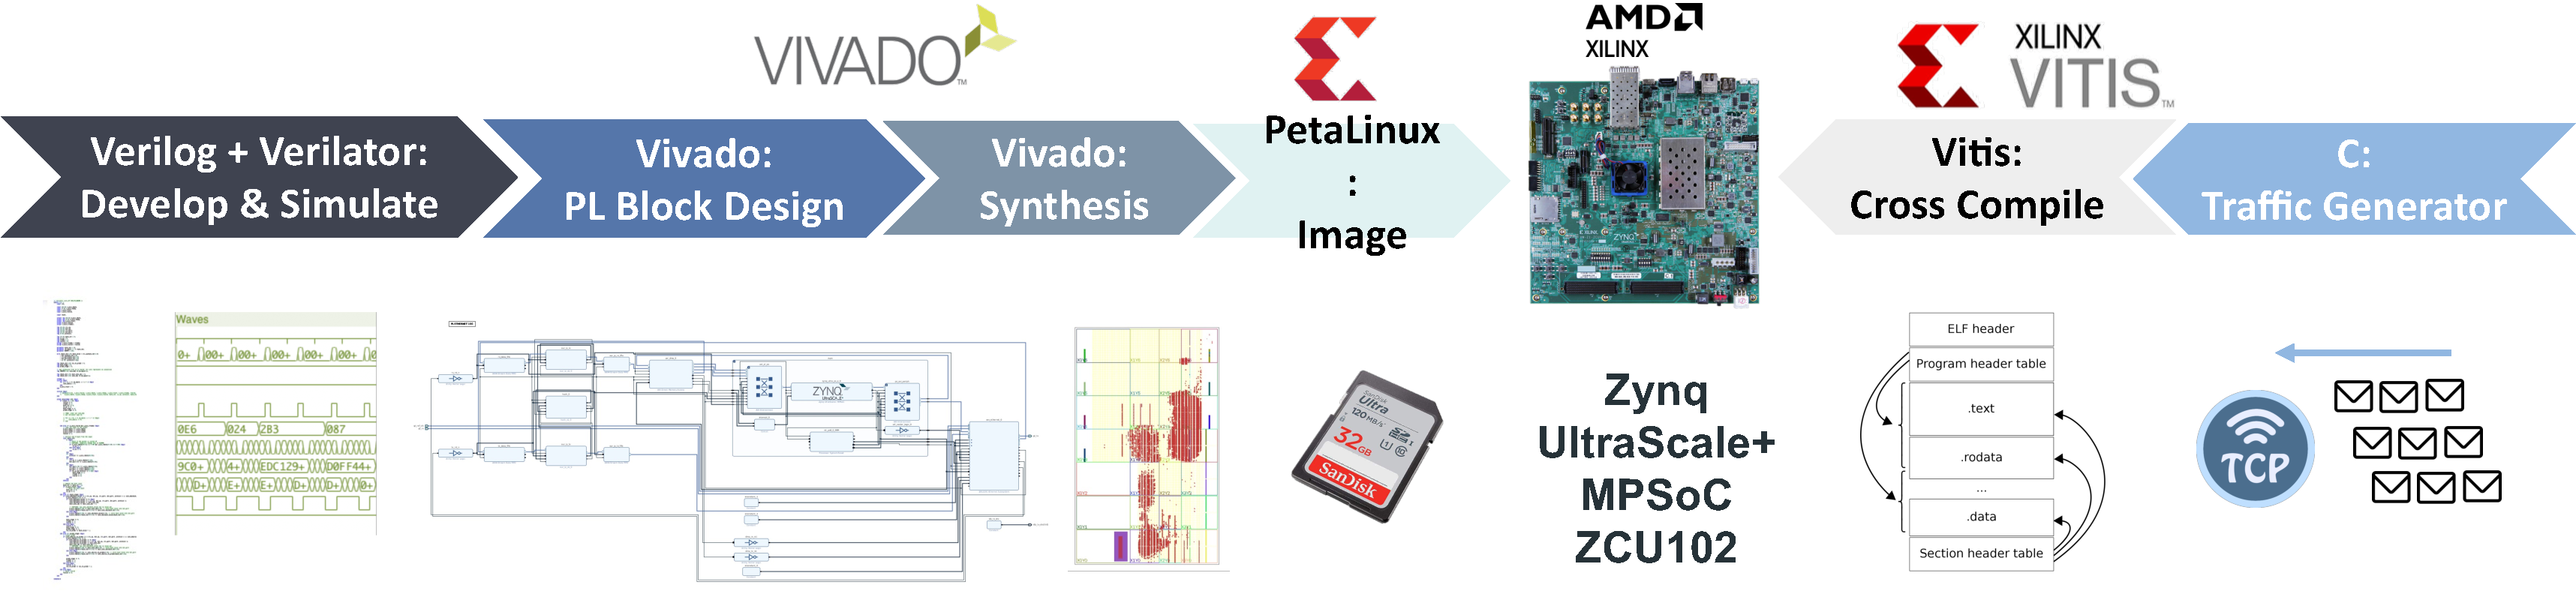
\includegraphics[width=500pt]{images/implworkflow.pdf}
    \caption{Our implementation workflow. }
    \label{fig:workflow}
    \Description{111}
\end{figure*}

We elaborate on our detailed implementation workflow, which includes Verilog design and testing, Vivado block design, Petalinux image building, testbed deployment, and Vitis cross-compile in this subsection. We use Vivado 19.02, Vitis 19.02, and Petalinux 19.02. Figure \ref{fig:workflow} shows our workflow.

\textbf{Hardware implementation and testing.} We use Verilog and Verilator to implement and test our design in about 300 lines of Verilog code and 1.5k lines of C++ code. 


\begin{table}
    \caption{ZCU102 Resource Consumption}
    \label{tab:res}
    \begin{tabular}{c|cccc}
      \toprule
        &LUT&FF&BRAM&DSP\\
      \midrule
      Origin & 18923 & 18315 & 139.5 & 0\\
      Ours (table size 1024) & 33373 & 47067 & 142.0 & 0\\

      \midrule
      Ours \slash Total Resource (\%) & 12.18 & 8.59 & 15.57 & 0\\

    \bottomrule
  \end{tabular}
\end{table}

\textbf{Vivado block design and synthesis.} We use Vivado to insert our Verilog implementation as custom IPs, and then synthesize, implement, and generate bitstream. Finally, we export the hardware to an \verb|.xsa| file. 
The resource consumption is shown in Table \ref{tab:res}.
The whole design (with table size 1024, original 10/25G Ethernet Subsystem included) consumes 12.18\% LUTs, 0.58\% LUTRAMs, 8.59\% FFs, 15.57\% BRAMs.
The delta of resource consumption between the original example and our modified design is 14464 LUTs, 13252 FF, 2.5 BRAM, and 0 DSP.
% Note that ConnectX-3 has the feature of L2, L3, and L4 checksum offloading. 
% We cannot disable it directly due to driver bugs.
Note that we use a custom Ethernet protocol number rather than \verb|0x0800| to prevent potential complexities such as NIC checksum-offloading and Linux kernel sanity check. Therefore, we do not need to insert CSU IP.

\textbf{Petalinux image building.} Petalinux is a tool to build tiny embedded Linux images.
The built image can be placed into an SD card to boot up the whole board. 
We build the images following the official tutorial in a Ubuntu 18.04 docker container over AMD Ryzen 7 7700 (4.8 Ghz full core). It takes up to several hours.

\textbf{Vitis cross-compilation.} We need to cross-compile the C++ source code since the CPUs on the board are ARM cores. Vitis provides cross-compile support for different Zynq platforms. The generated ELF file can be sent to the board via \verb|scp| directly.





% ○FPGA型号
% ○网络拓扑
% ○workflow,以及所有工具的版本
% ○soarx以及fpga上驱动版本号
% ○soarx、fpga上的Linux发行版以及内核版本
% ○网卡型号光纤线?光模组
% ○FPGA综合后占的资源
% ○代码行数
% ○
% ○表大小1024,MTU9000
% ○因为用了不同协议号,所以不需要插入CSU IP
% ○Detailed setting

% The whole design (with table size 1024, original 10/25G Ethernet Subsystem included) consumes 12.18\% LUTs, 0.58\% LUTRAMs, 8.59\% FFs, 15.57\% BRAMs.
% The delta of resource consumption between the original example and our modified design is 14464 LUTs, 13252 FF, 2.5 BRAM, and 0 DSP.

\section{Evaluation}

Hello
Here is our intro

\section{Discussion}
% ○discussion & future work:
% ■更好的实现方式:
% ●完全不经过PS
% ●more advanced NAT designs?
% ●
% ■更好的实验设计:
% ●FPGA性能弱对实验的影响
% ●软件NAT的实现方式对性能的影响
% ●实验不够详尽?还有什么关键的实验:

In this section, we will discuss some possible improvements in our system design and evaluation.

\textbf{Better evaluation method: bypassing PS.} Our evaluation result shows that the weak performance of ZCU102 PS hardware prevents it from fully investigating the potential of our hardware design. Thus, bypassing the PS part of the board may be a better choice to get precise evaluation results. To be specific, the received Ethernet packets should be sent back to another SFP interface after they are processed by our custom IPs in the PL logic, instead of passing them to those weak ARM CPUs.

\textbf{More efficient NAT design.} The NAT we implemented uses little resources at the cost of wasting more cycles. We can utilize the hardware parallelism by introducing structures like a full-associated cache in our NAT table which promises one cycle latency.

\textbf{Lack of connection state management.} A functional NAT should track connection states to release the NAT table entries in time. Due to the project time limit, we just discussed and came up with a possible design but did not implement this part. 

\section{conclusion}

Hello
Here is our intro

\section{Acknowledgement}
We would like to express our gratitude to Prof. Chenren Xu, the teaching assistants, and some senior colleagues for providing logistical support and valuable assistance.

\end{document}
\endinput
%%
%% End of file `sample-sigconf-biblatex.tex'.
